% begin module second-derivative-concavity
\begin{frame}
\begin{columns}[c]
\column{.5\textwidth}
\
\psset{xunit=0.9cm, yunit=0.9cm}
\begin{pspicture}(-0.5,-0.5)(4,3.8)
\psaxes[ticks=none, labels=none]{<->}(0,0)(-0.5,-0.5)(4,3.8)
%Function formula: 1/2+1/4 ((-1+x)^{2})+1/4 (x) 
\psplot[linecolor=red, plotpoints=1000]{-0.5}{4}{x 0.25 mul x -1 add 2 exp 0.25 mul add 0.5 add }

\rput(1, 2){$y=f(x)$}
%Function formula: -1/10 (x)+291/400 
\psplot[linecolor=blue, plotpoints=1000]{0}{0.6}{0.7275 x -0.1 mul add }
\psFullDot{0.3}{0.6975}

%Function formula: 2/5 (x)+131/400 
\psplot[linecolor=blue, plotpoints=1000]{1}{1.6}{0.3275 x 0.4 mul add } 
\psFullDot{1.3}{0.8475}

%Function formula: 9/10 (x)-229/400 
\psplot[linecolor=blue, plotpoints=1000]{2}{2.6}{-0.5725 x 0.9 mul add } 
\psFullDot{2.3}{1.4975}

%Function formula: 7/5 (x)-789/400 
\psplot[linecolor=blue, plotpoints=1000]{3}{3.6}{-1.9725 x 1.4 mul add } 
\psFullDot{3.3}{2.6475}
\end{pspicture} 
%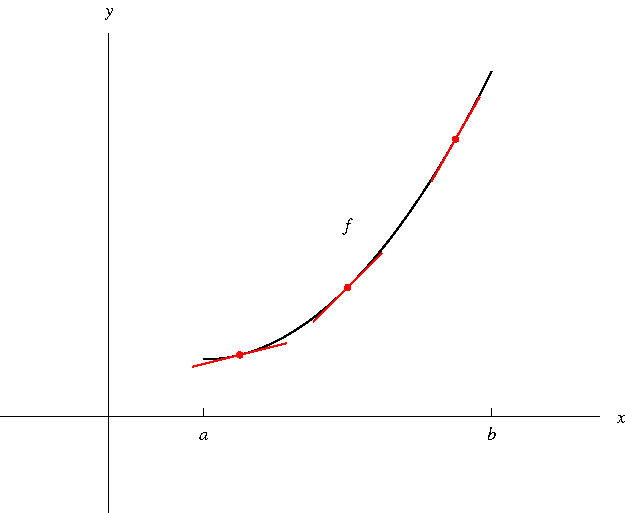
\includegraphics[height=3.5cm]{curve-sketching/pictures/04-03-concaveupe.pdf}%
\column{.5\textwidth}
\
\psset{xunit=0.9cm, yunit=0.9cm}
\begin{pspicture}(-0.5,-0.5)(4,3.8)
\psaxes[ticks=none, labels=none]{<->}(0,0)(-0.5,-0.5)(4,3.8)

\rput(2, 1){$y=g(x)$}
%Function formula: 11/4-1/4 ((-3+x)^{2})-1/4 (x) 
\psplot[linecolor=red, plotpoints=1000]{-0.5}{4}{x -0.25 mul x -3 add 2 exp -0.25 mul add 2.75 add }

%Function formula: 11/10 (x)+209/400 
\psplot[linecolor=blue, plotpoints=1000]{0}{0.6}{0.5225 x 1.1 mul add } 
\psFullDot{0.3}{0.8525}
%Function formula: 3/5 (x)+369/400 
\psplot[linecolor=blue, plotpoints=1000]{1}{1.6}{0.9225 x 0.6 mul add }
\psFullDot{1.3}{1.7025}
%Function formula: 1/10 (x)+729/400 
\psplot[linecolor=blue, plotpoints=1000]{2}{2.6}{1.8225 x 0.1 mul add 
}
\psFullDot{2.3}{2.0525}
%Function formula: -2/5 (x)+1289/400 
\psplot[linecolor=blue, plotpoints=1000]{3}{3.6}{3.2225 x -0.4 mul add }
\psFullDot{3.3}{1.9025}
\end{pspicture} 
%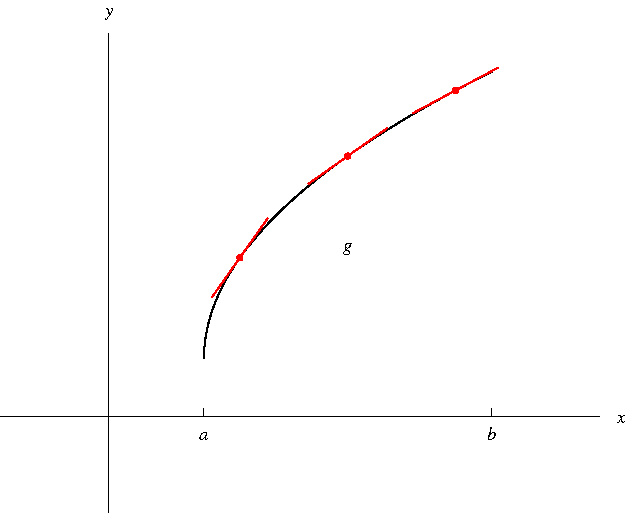
\includegraphics[height=3.5cm]{curve-sketching/pictures/04-03-concavedowne.pdf}%
\end{columns}
\begin{itemize}
\item  In the graph of $f$ the slopes of the tangent lines increase as we move from left to right.
\item<2->  This means $f'$ is an increasing function.
\item<3->  This means $f''$ is positive on $(a,b)$.
\item<4->  Similarly $g''$ is negative on $(a,b)$.
\end{itemize}
\uncover<5->{%
Concavity Test
\begin{enumerate}
\item  If $f''(x) > 0$ for all $x$ in $I$, then the graph of $f$ is concave up on $I$.
\item  If $f''(x) < 0$ for all $x$ in $I$, then the graph of $f$ is concave down on $I$.
\end{enumerate}
}%
\end{frame}
% end module second-derivative-concavity